\documentclass[12pt,titlepage,a4page , tikz , multi,table , svgnames,xcdraw]{article}
\usepackage{graphicx}
\usepackage[svgnames , table , xcdraw]{xcolor} 
\usepackage{fancyhdr}
\usepackage{fixltx2e}
 
\usepackage{hyperref}
\hypersetup{
    colorlinks=true,
    linkcolor=blue,
    filecolor=magenta,      
    urlcolor=cyan,
}

\usepackage{mathtools}
\usepackage{multirow}
\usepackage{graphicx}
\usepackage[ruled,vlined]{algorithm2e}
\usepackage{float}
\usepackage{enumitem}
\usepackage{listings }
\usepackage[a4paper, total={6in, 8in}]{geometry}
\usepackage{afterpage}
\usepackage{amssymb}
\usepackage{pdflscape}
\usepackage{lscape}
\usepackage{amsmath}
\usepackage{svg}
\usepackage[final]{pdfpages}
\usepackage{pgf, tikz}
\usetikzlibrary{arrows, automata}
\usetikzlibrary{shapes.multipart}


\DeclareMathOperator\arctanh{arctanh}

\usepackage[T1]{fontenc}
\usepackage{tikz}
\usepackage[utf8]{inputenc} % Required for inputting international characters
\usepackage{PTSerif} 

\usepackage{float}

\usepackage[Kashida]{xepersian}
\settextfont[
 BoldFont={XB Zar bold.ttf}
 ]{XB Zar.ttf}


\NewDocumentCommand{\codeword}{v}{
\texttt{\textcolor{blue}{#1}}
}
\DeclareFixedFont{\ttb}{T1}{txtt}{bx}{n}{12} % for bold
\DeclareFixedFont{\ttm}{T1}{txtt}{m}{n}{12}  % for normal


\definecolor{deepblue}{rgb}{0,0,0.5}
\definecolor{deepred}{rgb}{0.6,0,0}
\definecolor{deepgreen}{rgb}{0,0.5,0}

\hypersetup{citecolor=blue}

\newcommand\independent{\protect\mathpalette{\protect\independenT}{\perp}}
\def\independenT#1#2{\mathrel{\rlap{$#1#2$}\mkern2mu{#1#2}}}

% Python style for highlighting
\newcommand\pythonstyle{\lstset{
language=Python,
basicstyle=\ttm,
otherkeywords={self},             % Add keywords here
keywordstyle=\ttb\color{deepblue},
emph={MyClass,__init__},          % Custom highlighting
emphstyle=\ttb\color{deepred},    % Custom highlighting style
stringstyle=\color{deepgreen},
frame=tb,                         % Any extra options here
showstringspaces=false            % 
}}


% Python environment
\lstnewenvironment{python}[1][]
{
\pythonstyle
\lstset{#1}
}
{}

% Python for external files
\newcommand\pythonexternal[2][]{{
\pythonstyle
\lstinputlisting[#1]{#2}}}

\newenvironment{changemargin}[2]{%
\begin{list}{}{%
\setlength{\topsep}{0pt}%
\setlength{\leftmargin}{#1}%
\setlength{\rightmargin}{#2}%
\setlength{\listparindent}{\parindent}%
\setlength{\itemindent}{\parindent}%
\setlength{\parsep}{\parskip}%
}%
\item[]}{\end{list}}

% Python for inline
\newcommand\pythoninline[1]{{\pythonstyle\lstinline!#1!}}


\begin{document}

\begin{titlepage}

 \begin{center}
        
       \vspace*{0.5cm}

 \vspace{0.5cm}
       \textbf{ \Huge{به نام خدا} }
       \vspace{0.2cm}
       
       
\includegraphics[width=0.4\textwidth]{sharif1.png}
       
 	\vspace{0.3cm}
       \textbf{ \LARGE{طراحی سیستم‌های دیجیتال} }

 
   \vspace{0.3cm}
  \textbf{ \Large{ Single-Precision Floating Point Matrix Multiplier} }
   \vspace{0.3cm}
       
 
      \large \textbf{دانشکده مهندسی کامپیوتر}\\\vspace{0.2cm}
    \large   دانشگاه صنعتی شریف\\\vspace{0.25cm}
      
استاد:\\
    \textbf{{جناب آقای دکتر بهاروند}}

    \vspace{0.15cm}
    \noindent\rule[1ex]{\linewidth}{3pt}
    
    \vspace{0.5cm}
نام، نام خانوادگی و شماره دانشجویی اعضای گروه:\\

    
    \textbf{{رضا عبداله زاده - 97106132}}
        \vspace{0.05cm}
        
     
        \textbf{{فاطمه خاشعی - 97105899 }}
        \vspace{0.05cm}
        
        \textbf{{عرشیا اخوان - 97110422 }}
        \vspace{0.05cm}
        
           \textbf{{مجید طاهرخانی}}
        \vspace{0.05cm}
        
        
        \textbf{{رضا امینی}}
        \vspace{0.05cm}
        
       \textbf{{علی بالاپور - 97101326}}
        \vspace{0.05cm}


\end{center}
\end{titlepage}

\newpage
\pagestyle{fancy}
\fancyhf{}
\fancyfoot{}

\cfoot{\thepage}
\chead{پروژه پایانی}
\rhead{Matrix Multiplication}
\lhead{طراحی سیستم‌های دیجیتال}

\tableofcontents

\newpage

\section{مقدمه}

\subsection{چکیده}
عملیات ضرب دو ماتریس با اعداد اعشاری با دقت یگانه
\lr{(Single Precision Floating Point)}
امروزه کاربردهای بسیار زیادی در حوزه های مختلف علوم کامپیوتر از جمله هوش مصنوعی و یادگیری عمیق دارد. در این پروژه می خواهیم با استفاده از الگوریتم های داده شده و مدارهای ضرب و جمع 
\lr{Floating Point  (FP)}
، مداری برای انجام ضرب ماتریسی ارائه دهیم.


\subsection{تعریف و تاریخچه مختصر}
عملیات ضرب ماتریسی یکی از مهمترین عملیات های موجود در جبر خطی و ریاضیات می باشد. در ضرب ماتریسی، دو ماتریس با ابعاد 
\lr{n*m} 
و
\lr{m*k} در یکدیگر ضرب می شوند و یک ماتریس
\lr{n*k} حاصل می شود. شرط عملی بودن ضرب ماتریس این است که تعداد ستون های ماتریس اول با تعداد سطر های ماتریس دوم برابر باشد. در صورتی که 
\lr{A} 
و
\lr{B}
دو ماتریس با شرایط گفته شده باشند، حاصل ضرب ماتریسی به صورت 
\lr{AB}
نشان داده می شود. \cite{wikipedia}

\begin{center}
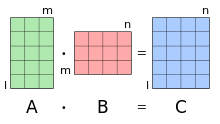
\includegraphics[scale=1]
    {Images/Introduction/Matrix_multiplication_overview.png}\\
\end{center}


در این پروژه ما به ضرب ماتریس هایی می پردازیم که درایه هایشان، اعداد اعشاری ممیز شناور با دقت یگانه و یا 
\lr{Single Precision Floating Point} می باشند. عملیات روی اعداد ممیز شناور 
\lr{(floating point)} به طور گسترده ای در پردازش های علمی مورد استفاده قرار می گیرد. سازمان 
\lr{IEEE} برای عملیات های ممیز شناور یک استاندارد کلی به نام 
\lr{IEEE-754} تعیین کرده است. در این پروژه، برای بدست آوردن حاصل ضرب دو ماتریس با درایه های اعشاری ممیز شناور، لازم است که از جمع و ضرب 
\lr{FP}
استفاده شود. در قسمت عملکرد، ضرب و جمع 
\lr{FP}
مورد بررسی واقع می شود. اما قبل از بررسی جمع و ضرب 
\lr{FP}
بهتر است با خود اعداد اعشاری ممیز شناور آشنا شویم. \\ 
در محاسبات عددی، از ممیز شناور ، به عنوان تقریبی برای پشتیبانی از توازن بین دامنه و دقت محاسبه استفاده می‌شود. به همین دلیل، محاسبات ممیز شناور اغلب در سیستم‌هایی یافت می‌شود که اعداد بسیار کوچک و بسیار بزرگی را شامل می‌شوند که نیازمند پردازش سریع هستند. یک عدد، به طور کلی، تقریبا از تعداد ثابتی از ارقام 
\lr{significand} و یک توان در پایه ثابت تشکیل می شود؛ این پایه معمولا 2، 10و یا ۱۶ است. یعنی: 

$$\text{significand} * \text{base}^{\text{exponent}}$$
منظور از ممیز شناور، این است که ممیز اعشاری عدد، می تواند شناور باشد. یعنی می توان آن را در هر قسمتی از عدد قرار داد. در نتیجه می توان ممیز شناور را نوعی نمادگذاری علمی تلقی کرد. از سیستم ممیز شناور می توان برای نشان دادن مقادیر بسیار زیاد و یا بسیار کم استفاده کرد. برای مثال می توان از این سیستم برای نمایش فاصله بین کهکشان ها یا فاصله بین عناصر موجود در هسته اتم استفاده کرد. \\
نمایش دقیق تر این شیوه به صورت زیر می باشد:

\begin{center}
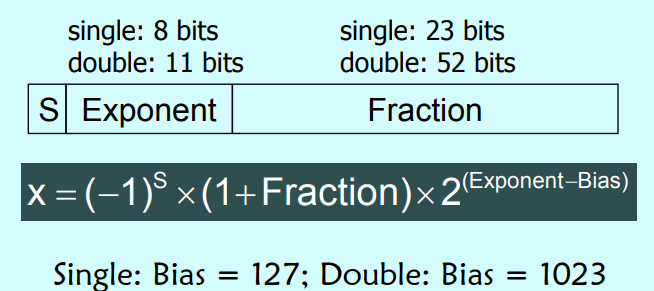
\includegraphics[scale=0.8]
    {Images/Introduction/FP_overview.png}\\
\end{center}
لازم به ذکر است که ما در این پروژه، از حالت Single استفاده می کنیم. \\

در طول سال های متمادی، انواع مختلفی از نمایش ممیز شناور برای محاسبات عددی در کامپیوتراستفاده شده است. در سال 1985، استاندارد 
\lr{IEEE 754} برای محاسبات ممیز شناور ثبت شد.  اين استاندارد واگرايي شيوه های به كار رفته براي نمايش مميز شناور را كاهش داد و امروزه اکثر کامپیوترها، از این استاندارد تبعیت می کنند. واحد اندازه گیری سرعت عملیات های ممیز شناور، 
\lr{FLOPS}
می باشد امروزه اکثر پردازنده های مدرن دارای یک واحد ممیز شناور برای انجام عملیات روی اعداد ممیز شناور می باشند. \cite{wikipediaFP}

نکته قابل توجه این است که پردازنده های نسل جدید (مخصوصا پردازنده های گرافیکی مانند سری 
\lr{RTX} شرکت 
\lr{Nvidia}) دارای واحد پردازشی مجزایی برای محاسبات ماتریسی می باشند. به این واحد های پردازشی، 
\lr{TPU} یا 
\lr{Tensor Processing Unit}
گفته می شود. البته به این پردازشگرها، هسته های تنسور 
\lr{(Tensor Cores)} هم گفته می شود. هسته های تنسور به طور خلاصه برای محاسبات ماتریسی کاربرد دارند و در زمینه هوش مصنوعی و یادگیری عمیق کاربردهای فراوانی دارند. یکی از مهمترین و کاربردی ترین وظایف چنین هسته هایی، ضرب ماتریسی می باشد. پس داشتن الگوریتم مناسب برای پیاده سازی ضرب ماتریس برای ساخت چنین واحدهای پردازشی ای، ضروری می باشد. \cite{wikipediaTPU} \cite{Tensor}



\subsection{نحوه عملکرد کلی}
\subsubsection{ساختار کلی}
	
    شرط پذیرا بودن ضرب دو ماتریس، یکسان بودن تعداد ستون‌های ماتریس اول (ماتریس سمت چپ) و تعداد سطرهای ماتریس دوم (ماتریس سمت راست) می باشد. برای مثال، دو ماتریس زیر را در نظر بگیرید. 

\begin{center}
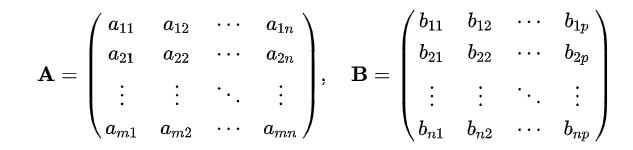
\includegraphics[scale=0.8]
    {Images/Introduction/mat_mult_1.png}\\
\end{center}

با توجه به این که ماتریس A دارای ابعاد m*n و ماتریس B دارای ابعاد n*p می باشد، پس ضرب این دو ماتریس پذیراست. فرض کنید حاصل ضرب ماتریسی این دو، ماتریسی به نام C می باشد که به شکل زیر است:
	
\begin{center}
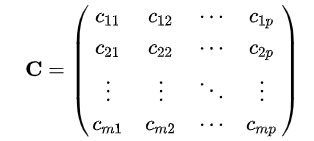
\includegraphics[scale=0.8]
    {Images/Introduction/mat_mult_2.png}\\
\end{center}

	ماتریس C دارای m سطر (تعداد سطر های ماتریس A) و دارای p  ستون (تعداد ستون های ماتریس B) می باشد. هر یک از درایه های ماتریس C از رابطه زیر به دست می آیند.

\begin{center}
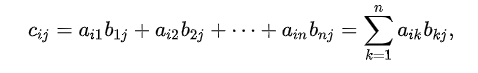
\includegraphics[scale=0.8]
    {Images/Introduction/mat_mult_3.png}\\
\end{center}

	به عبارت دیگر، سطر i ام ماتریس A و ستون j ام ماتریس B به عنوان یک وکتور(بردار) در نظر گرفته می شوند و حاصل ضرب داخلی این دو وکتور در درایه ij ماتریس C قرار می گیرد. در نهایت حاصلضرب ماتریسی دو ماتریس A و B که به صورت AB نشان داده می شود، به صورت زیر است:

\begin{center}
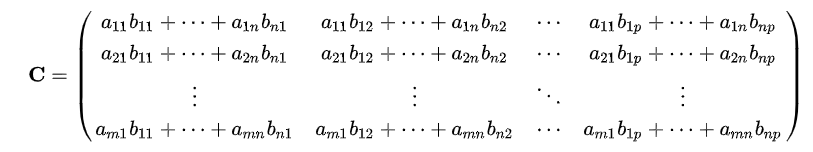
\includegraphics[scale=0.6]
    {Images/Introduction/mat_mult_4.png}\\
\end{center}

در قسمت های قبلی، اشاره شد که درایه های ماتریس، از جنس اعداد اعشاری ممیز شناور با دقت یگانه می باشند. برای محاسبه هر درایه ماتریس C، به تعدادی ضرب و جمع بین این اعداد، نیاز هست. لازم به ذکر است که ضرب و جمع این نوع اعداد، با ضرب و جمع اعداد معمولی و عادی، تفاوت دارد. در دو بخش بعدی به بررسی ضرب و جمع FP می پردازیم.

\subsubsection{جمع FP}
	همان گونه که اشاره شد، جمع اعداد 
    \lr{FP} دشوارتر از جمع اعداد صحیح می باشد و الگوریتم خاص خود را دارد. برای جمع دو عدد 
    \lr{a} و  
    \lr{b} که به صورت ممیز شناور می باشند و 
    \lr{a < b}
    ، داریم: \\
	1 - ابتدا توان های دو عدد را یکسان می کنیم. برای این کار، عدد کوچکتر یعنی a به سمت راست شیفت داده می شود. \\
	2 - مقادیر  دو عدد با هم جمع می شوند. \\
	3 - حاصل جمع، نرمال می شود. \\
	4 - 
    \lr{overflow} و یا 
    \lr{underflow} شدن حاصل جمع را بررسی می شود. \\
	5 - حاصل جمع گرد می شود.\\ 
	در صورتی که عدد نرمال نباشد، مراحل 3 تا 5 دوباره تکرار می شوند.
	رویه کلی انجام این کار در شکل زیر آمده است.

\begin{center}
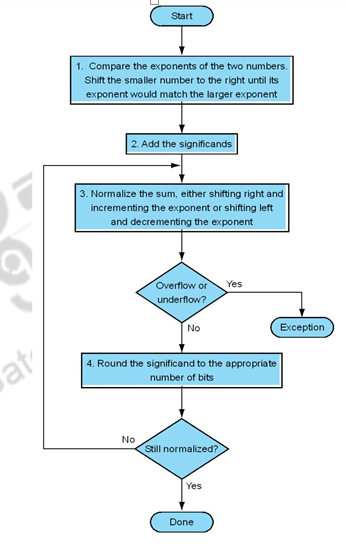
\includegraphics[scale=0.8]
    {Images/Introduction/Floating_point_sum.png}\\
\end{center}

برای مثال می‌خواهیم دو عدد 
$8.70 * 10^{-1}$
و 
$9.95*10^1$
را با یکدیگر جمع کنیم. ابتدا توان‌های دو عدد را باهم یکسان می کنیم. برای این کار، توان عدد کوچکتر را با توان عدد بزرگتر یکسان می کنیم. یعنی :
$$0.087*10^1 + 9.95*10^1$$
سپس این دو عدد را با یکدیگر جمع می زنیم و آن را نرمال می کنیم:
$$0.087 + 9.95 = 10.037 * 10^1$$
$$10.037*10^1 = 1.0037*10^2$$
و درنهایت حاصل را گرد می نماییم.
$$1.004 * 10^2$$

\cite{Floating_Point_Operationss} \cite{FPArithmatic}

\subsubsection{ضرب FP}
1 - ابتدا توان ها باهم جمع می شوند. \\
2 - مقادیر 
\lr{significand} در همدیگر ضرب می شوند. \\
3 - اعداد نرمال می شوند و سپس 
\lr{overflow} ویا 
\lr{underflow} شدن عدد حاصل، بررسی می شود. \\
4 - اعداد گرد می شوند. \\
در صورتی عدد نرمال نباشد، مراحل 3 و 4 تکرار می شود. \\
5 - علامت عدد تعیین می شود. \\
	رویه کلی الگوریتم ضرب 
    \lr{FP} با دقت یگانه، در فلوچارت زیر نیز مشخص می باشد.

\begin{center}
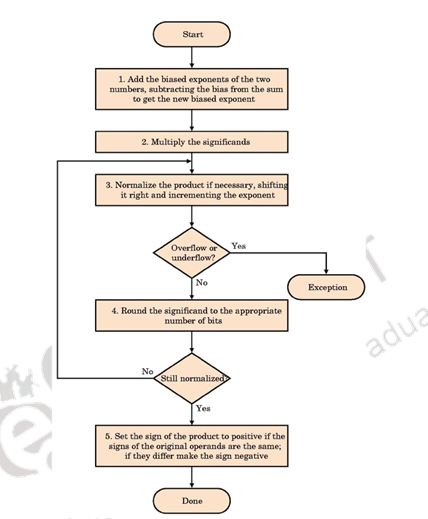
\includegraphics[scale=0.8]
    {Images/Introduction/Floating_point_mult.png}\\
\end{center}

برای مثال می‌خواهیم حاصلضرب دو عدد اعشاری با ممیزشناور 
$1.110 * 10^{10}$
و 
$9.200*10^{-5}$
را بدست آوریم. ابتدا توان های هردو عدد را یکسان می کنیم:
$$\text{\lr{new exponent}} = 10 - 5 = 5$$
سپس قسمت های اصلی اعداد را در یکدیگر ضرب می کنیم:
$$1.110 * 9.200 = 10.21200$$
سپس حاصل را نرمال کرده و رند می نماییم. در نتیجه خواهیم داشت:
$$1.021 * 10^6$$


\cite{Floating_Point_Operationss} \cite{FPArithmatic}

\subsection{کاربردها}
در گذشته، از ضرب ماتریسی به عنوان روشی برای راحت‌تر و واضح تر کردن محاسبات جبرخطی استفاده می شد. اما امروزه، ضرب ماتریسی یکی از مهمترین و پایه ای ترین عملیات ها در علوم ریاضیات، جبرخطی، فیزیک و علوم کامپیوتر می باشد. در ادامه به تعدادی از کاربردهای ضرب ماتریس می پردازیم.

\subsubsection{نگاشت خطی}
نگاشت خطی یا ترادیسش خطی، یک تابع بین دو فضای برداری است که دو عملیات جمع برداری و ضرب نرده‌ای را باقی نگه می‌دارد. این تابع همچنین رابطهٔ مستقیمی با عبارت عملگر خطی دارد که معمولاً در نگاشت‌های خطی از یک فضای برداری استفاده می‌شوند. از ضرب ماتریسی برای انجام نگاشت خطی، استفاده می شود. برای مثال، نگاشت خطی 
\lr{A}، یک ماتریس 
\lr{m*n} می باشد که برداری در فضای 
\lr{n} بعدی را به برداری در فضای 
\lr{m} بعدی تبدیل می کند. داریم:
\cite{wikipedia}

$$ x = \left( \begin{matrix} x_1 \\ x_2  \\
. \\
. \\
. \\
x_n \end{matrix} \right) $$
$$ A = \left( \begin{matrix} a_{11} & a_{12} & ... & a_{1n} \\
a_{21} & a_{22} & ... & . \\
a_{31} & a_{32} & ... & .\\
. & . \\
. && .\\
. &&& . \\
a_{m1} & a_{m2} & ... & a_{mn}
\end{matrix} \right) $$
$$ A(x) = \left( \begin{matrix} 
a_{11}x_1 + ... + a_{1n}x_n \\
a_{21}x_1 + ... + a_{2n}x_n  \\
. \\
. \\
. \\
a_{m1}x_1 + ... + a_{mn}x_n \end{matrix} \right) $$



\subsubsection{دستگاه معادلات خطی}
	برای حل دستگاه معادلات خطی، می توان از ضرب ماتریسی استفاده کرد.\cite{wikipedia}

\begin{center}
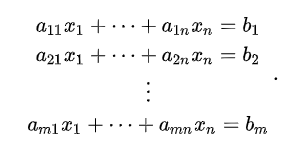
\includegraphics[scale=0.6]
    {Images/Introduction/EQ1.png}\\
\end{center}

\begin{center}
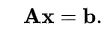
\includegraphics[scale=0.6]
    {Images/Introduction/EQ2.png}\\
\end{center}


\subsubsection{\lr{3D Projection}}
\lr{3D Projection}  یا 
\lr{Graphical Projection}
تکنیک طراحی ای است که برای نشان دادن یک شی سه بعدی از روی یک شی دو بعدی (سطح) استفاده می شود. روش های مختلفی برای اجرای این تکنیک وجود دارد. یک روش که 
\lr{Orthographic projection}
نام دارد، از ضرب ماتریسی برای اجرای این تکنیک استفاده می کند. \cite{wikipedia3DP}

\begin{center}
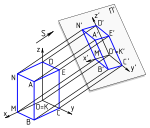
\includegraphics[scale=0.6]
    {Images/Introduction/3D_Projection.png}\\
\end{center}

\subsubsection{یادگیری عمیق}
	ضرب ماتریس یکی از مهمترین عملیات های مورد استفاده در یادگیری ماشین برای آموزش شبکه های عصبی می باشد. در هنگام آموزش مدل های عصبی عمیق، از ضرب ماتریس برای محاسبه و بروزرسانی وزن ها استفاده می شود. همچنین در مرحله تست نیز، برای بدست آوردن پاسخ نهایی، در هر لایه از عملیات ضرب ماتریسی استفاده می شود. بنابراین، درصورتی که بتوانیم مدار سریعتر و بهینه تری برای عملیات ضرب ماتریس داشته باشیم، می توانیم از الگوریتم های بهینه تری برای آموزش و تست شبکه های عصبی داشته باشیم و در نهایت مدل نهایی سریعتری خواهیم داشت. پس اهمیت بهینه بودن الگوریتم و مدار ضرب کننده ماتریس، در هوش مصنوعی و یادگیری عمیق، بسیار زیاد است.
    
\begin{center}
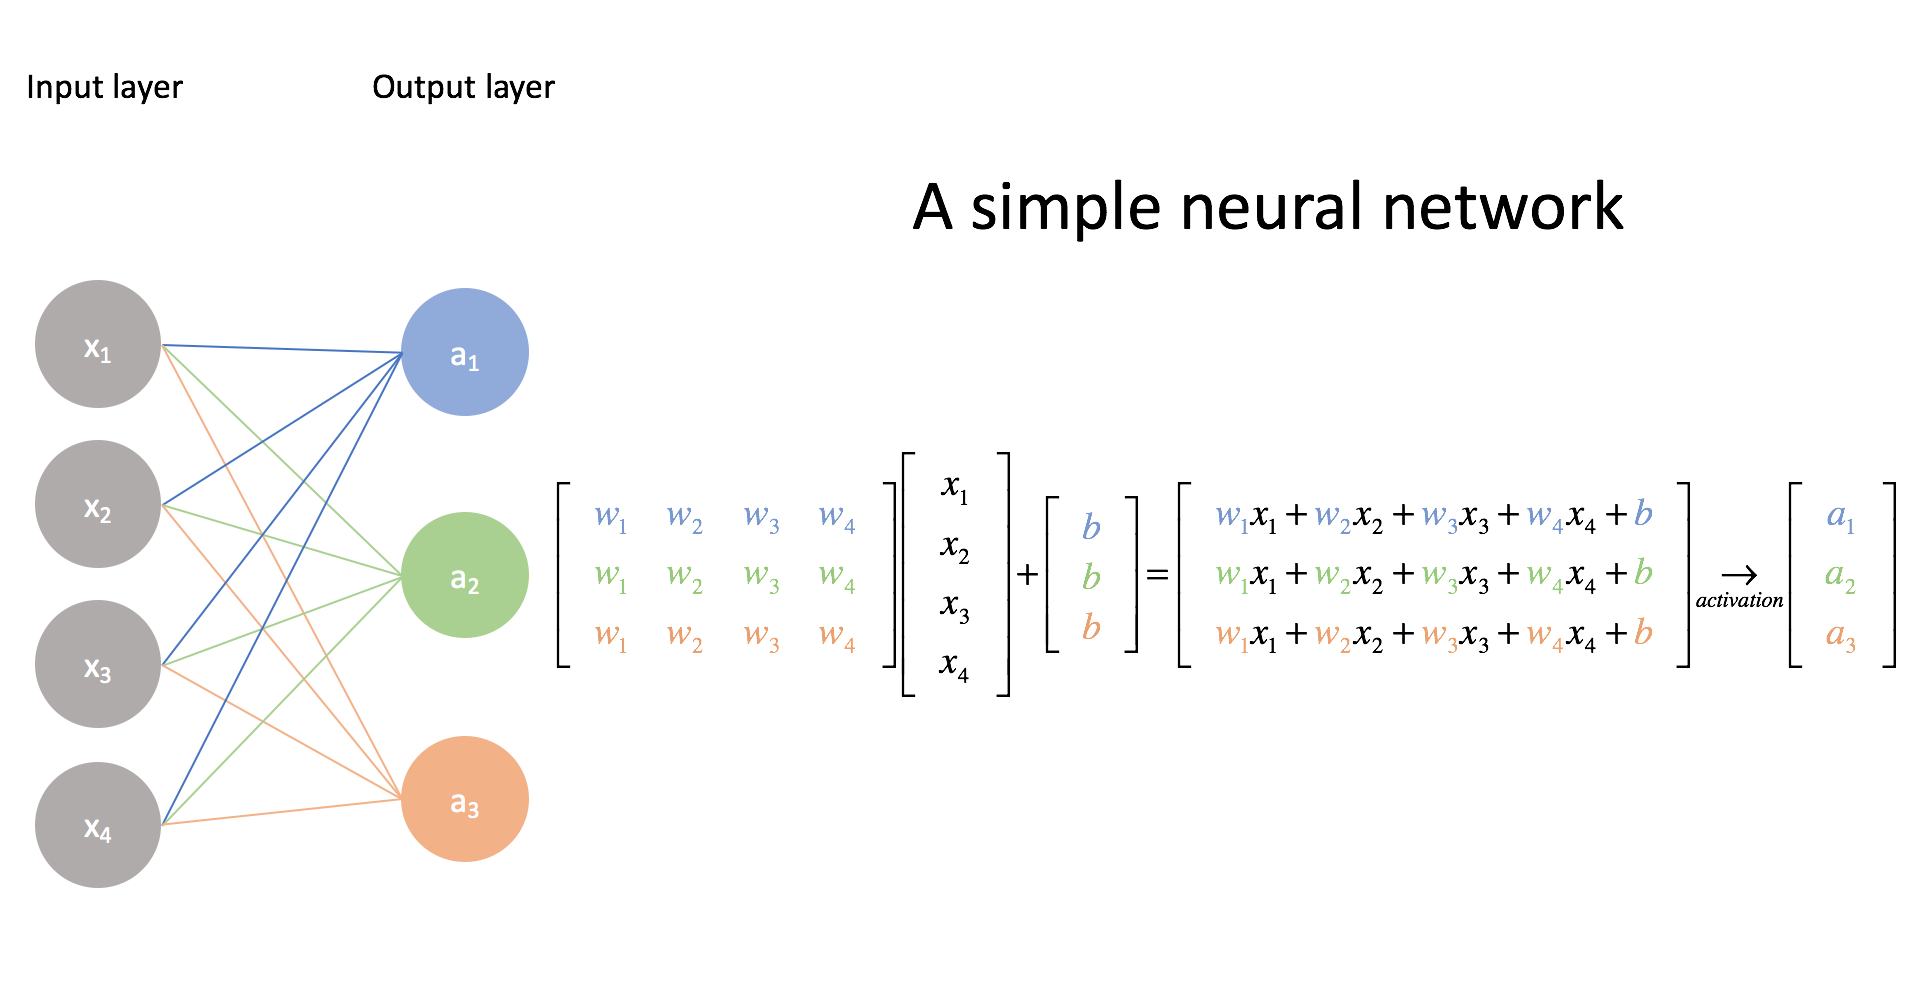
\includegraphics[scale=0.45] {Images/Introduction/Matrix_mult_deep_learning.png}\\
\end{center}


\newpage


\section{توصیف معماری سیستم}
\subsection{اینترفیس‌های سیستم و کلاک سیستم}
سیستم به طور کلی از 4 ماژول اصلی تشکیل شده است که این ماژول ها، به صورت تو در تو، از یکدیگر استفاده می کنند. هر ماژول واحد کنترل جداگانه خود را دارد و صرفا بین ماژول ها، سیگنال های کنترلی ای که مربوط به ماژول های دیگر است، رد و بدل می شود. این چهار ماژول اصلی به صورت زیر می‌باشند: \\ 
\lr{
\begin{itemize}
\item matrix\_multiplier
\item inner\_product
\item adder
\item multiplier
\end{itemize}
}
ماژول 
\lr{matrix\_multiplier} به نوعی ماژول اصلی سیستم ما می باشد و وظیفه دارد تا دو ورودی در قالب ماتریس را دریافت کرده و حاصل ضرب ماتریسی آن را محاسبه کند. برای این کار، به ازای هر سطر و ستون، از یک ماژول 
\lr{inner\_product}  استفاده می شود تا حاصل هر درایه، مشخص شود. همچنین در هر ماژول 
\lr{inner\_product}، از تعدادی ماژول 
\lr{adder} و 
\lr{multiplier} استفاده شده است که عمل جمع و ضرب 
\lr{FP} را انجام می‌دهند.
	
\subsubsection{پارامترها و ورودی‌ها}
	در ماژول 
\lr{matrix\_multiplier} پارامتر های 
\lr{m} و 
\lr{p} و 
\lr{n} و 
\lr{word\_width} به عنوان پارامترهای ورودی، به ماژول داده می شوند. این پارامترها به ترتیب نشان دهنده تعداد سطر ماتریس اول، تعدا ستون های ماتریس اول و سطرهای ماتریس دوم، تعداد ستون های ماتریس دوم و طول عدد هر درایه می باشند. همچنین به ترتیب، مقادیر پیش فرض 16 - 16 - 16 - 32 به این پارامترها داده شده است. البته لازم به ذکر است، همان گونه که در مقدمه بحث شد، برای این که ضرب دو ماتریس پذیرا باشد، باید حتما تعداد ستون های ماتریس اول با تعداد سطرهای ماتریس دوم برابر باشد. \\ 
	ورودی های اصلی این ماژول، دو ماتریس 
\lr{matrix\_A} و 
\lr{matrix\_B} و سیگنال 
\lr{start} و 
\lr{clk} می باشند. با توجه به این که نمی توان یک آرایه را به عنوان ورودی، به ماژول داد، پس هر کدام از ماتریس ها را به یک وکتور با سایز 
\lr{m*p*word\_width} (برای ماتریس اول) و با سایز 
\lr{p*n*word\_width} (برای ماتریس دوم) به عنوان ورودی می گیریم. یعنی در هر ماتریس همه سطرها را پشت سرهم قرار داده و آن هارا به صورت بیت به بیت ذخیره می کنیم. همچنین می دانیم هر عدد 32 بیت (یا به اندازه 
\lr{word\_width}) فضا را اشغال می کند. پس به راحتی می توان به هر عدد دسترسی داشت. سیگنال 
\lr{start} هم تعیین کننده شروع کار کل مدار می باشد. همچنین سیگنال 
\lr{clk} نیز کلاک کلی مدار می باشد. \\
	در ماژول 
    \lr{inner\_product}، پارامتر 
    \lr{number\_of\_element} نشان دهنده تعداد اعضای وکتور ها می باشد. در این ماژول ورودی های 
    \lr{In1, In2, clk, rst, start}  به ماژول داده می شود. 
    \lr{In1} و 
    \lr{In2} دو وکتور با سایز های برابر (
    \lr{element\_length * number\_of\_elements}) می باشند که مقادیر دو بردار ( به طور دقیق تر سطر ماتریس اول و ستون ماتریس دوم) در آن های ذخیره شده است. هدف این ماژول ضرب داخلی این دو بردار در هم می باشد. همچنین سیگنال های 
    \lr{rst} به معنای 
    \lr{reset} ماژول 
    \lr{inner\_product}، 
    \lr{clk} به معنای کلاک کلی مدار و 
    \lr{start}  به معنای شروع فرآیند ضرب داخلی، به عنوان ورودی به این ماژول داده شده است.
	ورودی ها و خروجی های دو ماژول 
    \lr{multiplier} و 
    \lr{adder} با یکدیگر یکسان می باشند. ورودی های این دو ماژول عبارتند از :
    \lr{input\_a, input\_b, input\_a\_stb, input\_b\_stb, output\_z\_ack,clk, rst}.
    دو ورودی 
    \lr{input\_a} و 
    \lr{input\_b} همان عملوندهای اصلی ما می باشند. ورودی های 
    \lr{stb} نشان دهنده این موضوع اند که آیا دو عملوند اصلی یعنی 
    \lr{input\_a} و 
    \lr{input\_b} آماده عملیات هستند یا خیر. در صورتی که هر دو سیگنال 
    \lr{stb} یک شوند، در این صورت عملیات ضرب یا جمع شروع می شود. ورودی 
    \lr{rst} و 
    \lr{clk}  نیز واضح می باشند.


\subsubsection{خروجی‌ها}
در ماژول 
\lr{matrix\_multiplier} یکی از خروجی ها، ماتریس خروجی یا همان 
\lr{matrix\_C} خواهد بود. این ماتریس، حاصل ضرب ماتریسی دو ماتریس ورودی 
\lr{matrix\_A} و 
\lr{matrix\_B} می باشد. همان گونه که در قسمت قبل نیز اشاره شد، با توجه به این که نمی توان آرایه در یک ماژول خروجی داد، پس مانند قسمت قبل عمل کرده و هر سطر را پشت سرهم قرار در یک وکتور با سایز 
\lr{m*n*word\_width} قرار می دهیم. این ماژول دو سیگنال خروجی با نام های 
\lr{done}  و 
\lr{ready} نیز دارد که به ترتیب نشان دهنده اتمام عملیات و آماده بودن ماژول برای دریافت ورودی می باشد. \\
	در ماژول 
    \lr{inner\_product} خروجی 
    \lr{out} و 
    \lr{done}  را داریم. 
    \lr{done}  نشان دهنده تمام شدن عملیات ضرب داخلی می باشد. 
    \lr{out}  نیز یک عدد 32 بیتی (به طور پیش فرض) می باشد که نشان دهنده حاصل ضرب داخلی است. \\ 
	در ماژول های  
    \lr{multiplier} و 
    \lr{adder} نیز خروجی های 
    \lr{output\_z، output\_z\_stb، input\_a\_ack و input\_b\_ack} را داریم. 
    \lr{output\_z} همان خروجی جمع و یا ضرب می باشد که سایز آن به طور پیش فرض برابر 32 بیت است. 
    \lr{output\_z\_stb} نیز اتمام عملیات ضرب و جمع را نشان می دهد.

\subsubsection{کلاک سیستم}
	همان گونه که در قسمت های بالا نیز اشاره شد، کلاک استفاده شده در هریک از ماژول ها، همان کلاک اصلی سیستم می باشد. 
	





\subsection{دیاگرام بلوکی سخت‌افزار}

\begin{center}
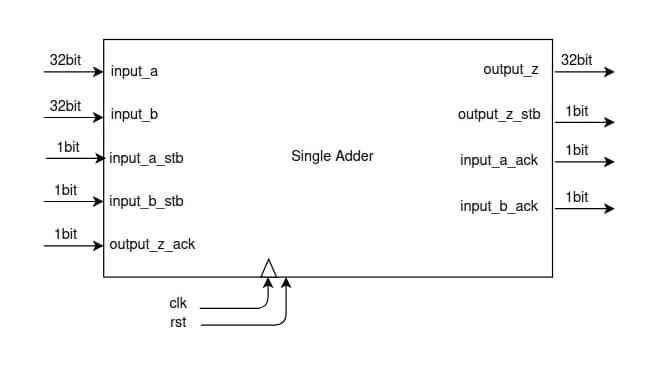
\includegraphics[scale=0.8] {Images/System Architecture/adder.jpg}\\
\caption{دیاگرام ماژول جمع‌کننده}
\end{center} 

\begin{center}
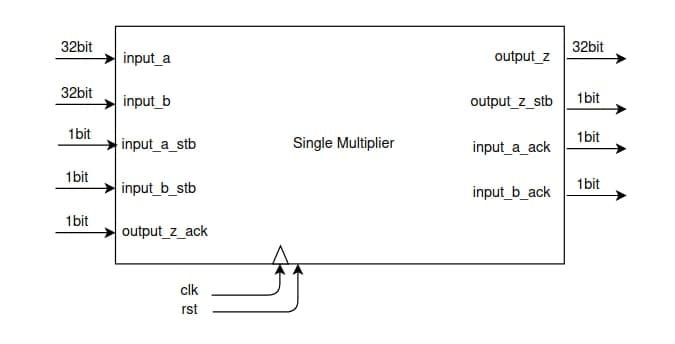
\includegraphics[scale=0.8] {Images/System Architecture/multiplier.jpg}\\
\caption{دیاگرام ماژول ضرب‌کننده}
\end{center} 

\begin{center}
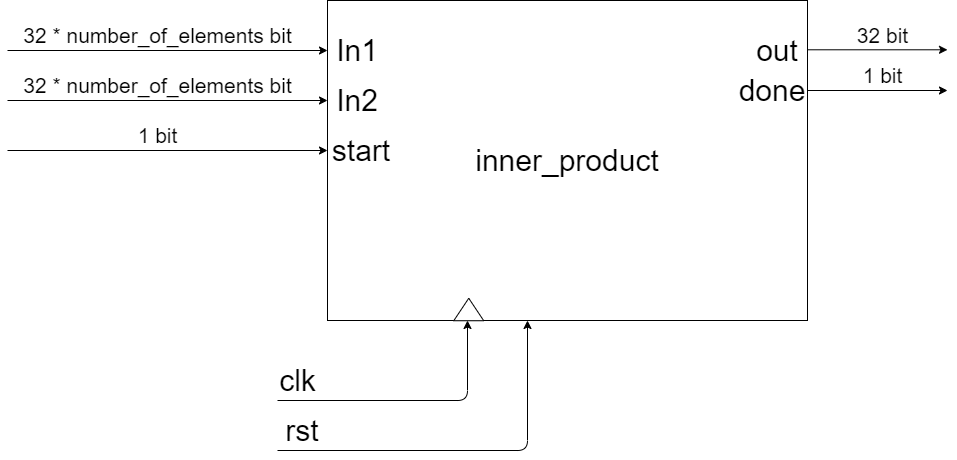
\includegraphics[scale=0.4] {Images/System Architecture/DSD_Project_inner_product_overview_diagram.png}\\
\caption{دیاگرام ماژول ضرب داخلی}
\end{center} 


\begin{center}
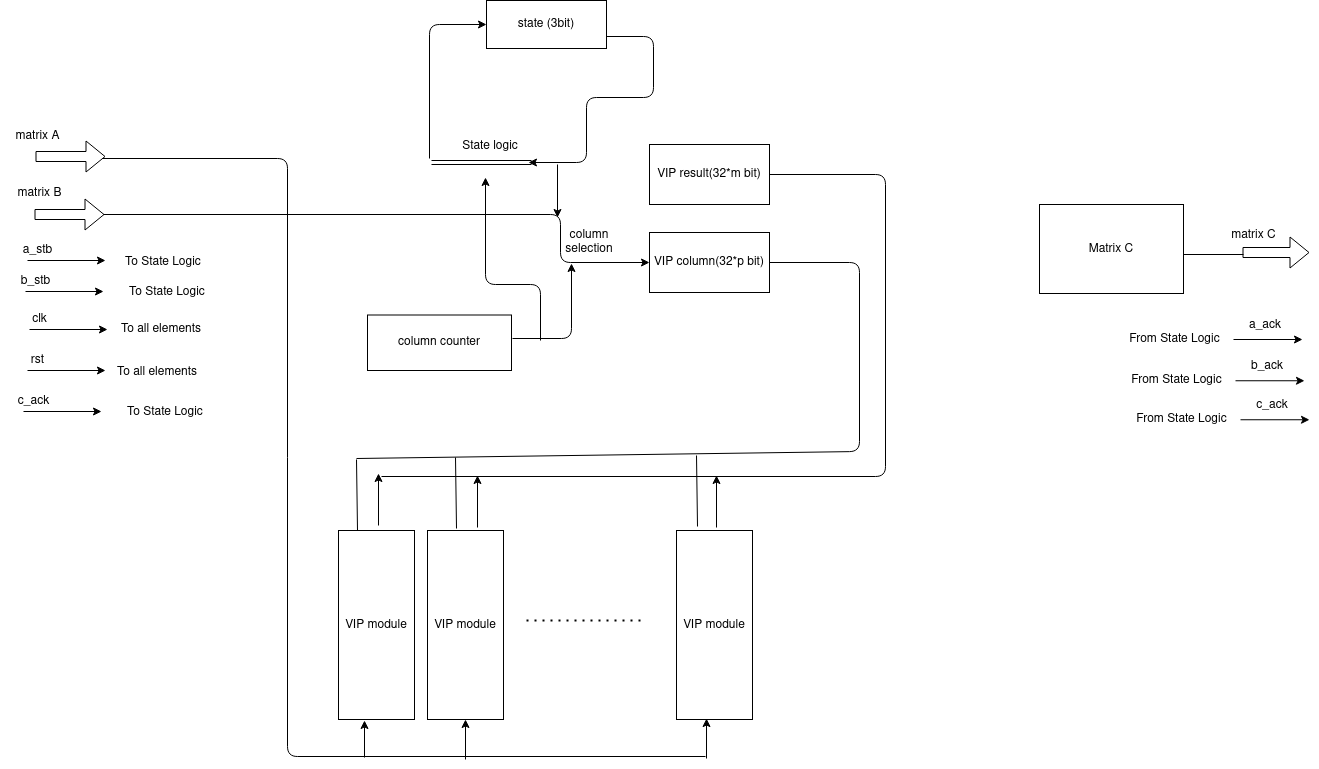
\includegraphics[scale=0.33] {Images/System Architecture/matrix multiplier.png}\\
\caption{دیاگرام کلی ماژول ضرب کننده دو ماتریس}
\end{center} 



\subsection{توصیف وظیفه ماژول‌های سخت‌افزار}
\subsubsection{\lr{Single Multiplier}}
همان‌گونه که در قسمت قبل اشاره شد، این ماژول دو عدد 32 بیتی ممیز شناور را به عنوان ورودی دریافت می‌کند و حاصلضرب این دو عدد را محاسبه می نماید. دو عددی ورودی 
\lr{a} و 
\lr{b} نام دارند و خروجی 
\lr{z} نام دارد. در ابتدای ماژول، استیت های مختلف به عنوان پارامتر مشخص شده اند و تعدادی متغیر برای ذخیره سازی قسمت های مختلف اعداد (برای مثال توان های اعداد) در نظر گرفته شده است. استیت های ماژول به گونه زیر می باشند (در هر قسمت، عملیات انجام شده در هر استیت به طور خلاصه توصیف شده است.): 
\begin{itemize}
\item \lr{get\_a} \\
در این استیت، ماژول آماده است که ورودی اول از ماژول \lr{top} گرفته شود و در داخل متغیر \lr{a} قرار داده شود. پس از دریافت ورودی اول، سیگنال \lr{ack} به ماژول بالاتر فرستاده می شود و ماژول ضرب کننده به استیت دریافت ورودی دوم می‌رود.
\item \lr{get\_b} \\
این استیت مشابه استیت بالا می‌باشد. پس از دریافت ورودی دوم و ارسال سیگنال \lr{ack}، ماژول به استیت \lr{unpack} می رود.
\item \lr{unpack} \\
در این استیت، همانگونه که از اسم آن مشخص است، اعداد ورودی به چند قسمت تقسیم می‌شوند تا فرآیند ضرب عدد اعشاری، تسهیل شود. به ازای هر عدد اعشاری ورودی، 23 بیت کم ارزش به عنوان \lr{mantissa} جدا می‌شود. 8 بیت بعدی هر عدد نیز جدا شده و عدد 127 از آن کم می شود تا توان عدد یا \lr{exponent} محاسبه و در متغیر مخصوص خود، ذخیره شود. و در نهایت، بیت پرارزش نیز به عنوان علامت عدد در نظر گرفته شده و در متغیر مخصوص خود، ذخیره می‌شود. لازم به ذکر است که همه این عملیات‌ها، بر روی هر دو عدد انجام می‌شود.
\item \lr{special\_cases} \\
در این استیت، موارد خاصی که ممکن است به عنوان عدد ورودی، به ماژول داده شود، بررسی می گردد و اقدامات لازم برای ضرب چنین موارد خاصی، اتخاذ می‌گردد. برای مثال در این استیت چک می‌شود که آیا یکی از اعداد ورودی مقدار بینهایت دارد یا خیر. در صورت داشتن چینین مقداری، خروجی باید مقدار بینهایت باشد.
\item \lr{normalise\_a} \\
همانگونه که در مقدمه نیز ذکر شده است، فرآیند ضرب دو عدد اعشاری با فرمت ممیز شناور، با ضرب اعداد صحیح تفاوت دارد. در این استیت و استیت بعد، دو عدد ورودی، با توجه به این که کدام عدد شرایط لازم را ندارد، با شیفت دادن و کم کردن توان، نرمال می‌شوند.
\item \lr{normalise\_b} \\
عملکرد این استیت، مشابه استیت قبل می‌باشد. 
\item \lr{multiply\_0} \\
در این استیت، مقدار توان و علامت حاصل ضرب، یعنی متغیر \lr{z} مشخص می‌شود و ماژول آماده محاسبه قسمت اصلی حاصلظرب می‌شود.
\item \lr{multiply\_1} \\
در این استیت، قسمت \lr{mantissa} حاصلضرب با استفاده از متغیرهای کمکی ایجاد شده در استیت قبلی، محاسبه می‌شود.
\item \lr{normalise\_1 & 2} \\
در این دو استیت، مقدارحاصلضرب نرمال می‌شود.

\item \lr{round} \\
در این استیت، مقدار حاصلضرب، با توجه به شرایطی که دارد، گرد می‌شود تا آماده ماژول آماده تحویل دادن خروجی گردد.
\item \lr{pack} \\
در این استیت، 23 بیت کم ارزش \lr{mantissa} محاسبه شده، در 23 بیت کم ارزش متغیر خروجی اصلی قرار می‌گیرد. همچنین 8 بیت بعدی که نشان دهنده توان عدد حاصلضرب می‌باشد، نیز در جایگاه خود قرار میگیرد. و در نهایت، علامت عدد تعیین می شود. 
\item \lr{put\_z} \\
        در این استیت، که استیت نهایی نیز می‌باشد، حاصلضرب در متغیر خروجی ماژول قرار گرفته و سیگنال \lr{stb} نیز فعال می‌شود. پس از اتمام این استیت، ماژول به استیت اولیه بازمی‌گردد.
\end{itemize}




\subsubsection{\lr{Single Adder}}
همان‌گونه که در قسمت قبل اشاره شد، این ماژول دو عدد 32 بیتی ممیز شناور را به عنوان ورودی دریافت می‌کند و حاصل جمع این دو عدد را محاسبه می‌نماید. این ماژول شباهت بسیار زیادی به ماژول ضرب کننده دارد. دو عددی ورودی 
\lr{a} و 
\lr{b} نام دارند و خروجی 
\lr{z} نام دارد. در ابتدای ماژول، استیت های مختلف به عنوان پارامتر مشخص شده اند و تعدادی متغیر برای ذخیره سازی قسمت های مختلف اعداد (برای مثال توان های اعداد) در نظر گرفته شده است. استیت های ماژول به گونه زیر می باشند (در هر قسمت، عملیات انجام شده در هر استیت به طور خلاصه توصیف شده است.): 
\begin{itemize}
\item \lr{get\_a} \\
در این استیت، ماژول آماده است که ورودی اول از ماژول \lr{top} گرفته شود و در داخل متغیر \lr{a} قرار داده شود. پس از دریافت ورودی اول، سیگنال \lr{ack} به ماژول بالاتر فرستاده می شود و ماژول جمع کننده به استیت دریافت ورودی دوم می‌رود.
\item \lr{get\_b} \\
این استیت مشابه استیت بالا می‌باشد. پس از دریافت ورودی دوم و ارسال سیگنال \lr{ack}، ماژول به استیت \lr{unpack} می رود.
\item \lr{unpack} \\
در این استیت، همانگونه که از اسم آن مشخص است، اعداد ورودی به چند قسمت تقسیم می‌شوند تا فرآیند جمع عدد اعشاری، تسهیل شود. به ازای هر عدد اعشاری ورودی، 23 بیت کم ارزش به عنوان \lr{mantissa} جدا می‌شود. 8 بیت بعدی هر عدد نیز جدا شده و عدد 127 از آن کم می شود تا توان عدد یا \lr{exponent} محاسبه و در متغیر مخصوص خود، ذخیره شود. و در نهایت، بیت پرارزش نیز به عنوان علامت عدد در نظر گرفته شده و در متغیر مخصوص خود، ذخیره می‌شود. لازم به ذکر است که همه این عملیات‌ها، بر روی هر دو عدد انجام می‌شود.
\item \lr{special\_cases} \\
در این استیت، موارد خاصی که ممکن است به عنوان عدد ورودی، به ماژول داده شود، بررسی می گردد و اقدامات لازم برای ضرب چنین موارد خاصی، اتخاذ می‌گردد. برای مثال در این استیت چک می‌شود که آیا یکی از اعداد ورودی مقدار بینهایت دارد یا خیر. در صورت داشتن چینین مقداری، خروجی باید مقدار بینهایت باشد.
\item \lr{align} \\
در این استیت، با توجه به این که کدام یک از دو عدد ورودی بزرگتر است، توان عدد کوچکتر برابر با عدد بزرگتر قرار داده می‌شود تا توان‌های دو عدد باهم برابر شوند. همچنین عملیات شیفت \lr{mantissa} عدد کوچکتر نیز در این استیت انجام می‌شود. پس از هم توان کردن دو عدد ورودی، به مرحله اصلی جمع می‌رویم.


\item \lr{add\_0 & add\_1} \\
در این استیت، عملیات جمع انجام می‌شود. ابتدا علامت های دوعدد چک می شوند و سپس با توجه به علامت‌های دو عدد، عمل جمع \lr{mantissa} انجام می‌شود. 
در نهایت به استیت نرمال کردن حاصل جمع،، می‌رویم.

\item \lr{normalise\_1 & normalize\_2} \\
در این دو استیت، حاصل جمع دو عدد ورودی، با شیفت دادن و کم کردن توان، نرمال می‌شوند.

\item \lr{round} \\
 مقدار جمع،  با توجه به شرایطی که دارد، گرد می‌شود تا آماده ماژول آماده تحویل دادن خروجی گردد

\item \lr{pack} \\
در این استیت، 23 بیت کم ارزش \lr{mantissa} محاسبه شده، در 23 بیت کم ارزش متغیر خروجی اصلی قرار می‌گیرد. همچنین 8 بیت بعدی که نشان دهنده توان عدد حاصل‌جمع می‌باشد، نیز در جایگاه خود قرار میگیرد. و در نهایت، علامت عدد تعیین می شود. 
\item \lr{put\_z} \\
        در این استیت، که استیت نهایی نیز می‌باشد، حاصل جمع در متغیر خروجی ماژول قرار گرفته و سیگنال \lr{stb} نیز فعال می‌شود. پس از اتمام این استیت، ماژول به استیت اولیه بازمی‌گردد.
\end{itemize}




\subsubsection{\lr{Vector Inner Product}}
وظیفه این ماژول اعمال ضرب داخل دو بردار داده شده است.
برای انجام این کار از الگوریتم ساده‌ی ضرب تک تک درایه ها در هم و سپس جمع این مقادیر استفاده می‌شود.
ابتدا طبق قواعد 
\lr{handshake} ورودی های 
\lr{a} و 
\lr{b} شامل دو بردار از مقادیر 
\lr{floating-point}
(به تعداد \lr{number\_of\_elements)} که برابر تعداد درایه‌های سطری یا ستونی است)
که 32 
\lr{bit} هستند، ورودی گرفته می‌شود و سپس اعمال ضرب تک به تک و خروجی دادن انجام می‌شود.
پس از اتمام کار عدد ۳۲بیتی حاصل از جمع به عنوان خروجی داده می‌شود.

در این ماژول به طور دقیق مقدار
\[a_i * b_i = c_i\]
به کمک 
\lr{single Multiplier} محاسبه می‌شود و در یک بردار c ذخیره می‌شود.
سپس به کمک ماژول 
\lr{single Adder} هر کدام از 
\lr{c\textsubscript{i}}
ها با یک مقدار 
\lr{accumulator} جمع شده و در نهایت پس از پایدار شدن به عنوان خروجی داده می‌شود.

در ابتدا در یک
\lr{ generate block}
یک حلقه به اندازه 
\lr{number\_of\_elements}
برای ضرب کننده ها
داریم که بصورت هم زمان تمام درایه های دو وکتور را بطور متناظر در هم ضرب میکنند و حاصل را در درایه ی نظیر در آرایه 
\lr{temp1\_vector}
میریزیم سپس یک متغیر به نام
\lr{ temp\_res }
داریم که در ابتدا برابر صفر است و با تمام خانه های آرایه
\lr{temp1\_vector}
جمع میشود تا حاصل نهایی را خروجی دهد.
برای انجام این فرآبند‌ها ۶ 
\lr{state} 
وجود دارد که در ابتداری ماژول با اعداد ۰ تا ۵ مقداردهی شده‌اند.
\lr{state}
 های ماژول به گونه زیر می باشند (در هر قسمت، عملیات انجام شده در هر 
 \lr{state}
 به طور خلاصه توصیف شده است.): 
 
 
\begin{itemize}

\item \lr{state\_idle} \\
در ابتدا در اینجا قرار داریم و اگر ورودی 
\lr{start}
یک و ورودی 
\lr{vip\_done}
صفر باشد به استیت بعدی می‌رویم.

\item \lr{state\_mult\_elements} \\
در این مرحله فرایند ضرب را شروع می‌کنیم
(\lr{stb} 
هارا یک می‌کنیم، این سیگنال ها در در تمامی ضرب کننده ها یکی است) و ورودی ها وارد ضرب کننده ها می‌شوند.

\item \lr{state\_wait\_for\_mult} \\
در این مرحله انقدر منتظر می‌مانیم تا تمام 
\lr{stb} 
های خروجی در تمام ضرب کننده ها یک شود و وقتی این اتفاق افتاد و یعنی خروجی آماده بود و خروجی درون خانه های آرایه 
\lr{temp1\_vector}
ریخته شد، به مرحله بعد می‌رویم.

\item \lr{state\_add\_elements} \\
ما یک 
\lr{adder}
داریم و به ترتیب به عنوان ورودی 
\lr{temp\_res} 
و یکی از درایه های 
\lr{temp1\_vector}
را ورودی می‌دهیم به آن و خروجی را در 
\lr{temp\_res} 
می‌ریزیم، و در متغیر 
\lr{index} 
شماره خانه‌ی فعلی از 
\lr{temp1\_vector}
را نگه می‌داریم. در این حالت
\lr{stb} 
هارا یک می‌کنیم و ورودی ها به 
\lr{adder} 
می‌روند و به مرحله ی بعد برای گرفتن خروجی می‌رویم.

\item \lr{state\_wait\_for\_add} \\
در حالت انقدر می‌مانیم تا 
\lr{stb} 
خروجی یک شود و وقتی یک شد خروجی را می‌گیریم و در 
\lr{temp\_res} 
می‌ریزیم و سپس
\lr{index}
را یکی زیاد می‌کنیم (در اول قسمت قبل شرط پایان چک می‌شود یعنی وقتی که 
\lr{index}
برابر 1+
\lr{number\_of\_elements}
شود.)

\item \lr{state\_out\_is\_ready} \\
مرحله ی اخر است که 
\lr{vip\_done} 
را یک می‌کنیم و به حالت صفر برمی‌گردیم.
(
\lr{state\_idle}
)

\end{itemize}


\subsubsection{\lr{Matrix Multiplier}}
این ماژول، ماژول اصلی مدار را تشکیل می‌دهد و هدف آن محاسبه ضرب دو ماتریس داده شده است.
برای انجام این کار از یک بخش ترکیبی برای برای محاسبه حاصل ضرب در هر ستون و یک بخش ترتیبی برای تعمیم بخش ترکیبی به تمام ستون ها استفاده می‌شود و الگوریتم اجرای آن الگوریتم معمول محاسبه ضرب داخلی ردیف های ماتریس نخست و ستون های ماتریس دوم است.
 دو ورودی شامل دو ماتریس 
 \lr{A} و 
 \lr{B} در قالب دو بردار به ابعاد تعداد درایه های هر ماتریس ضرب در تعداد بیت هر درایه با پیروی از قوانین 
 \lr{handshake} ورودی داده می‌شود و سپس با محاسبه ضرب این دو ماتریس ، مقدار Cدرقالب یک بردار مشابه ورودی ها به عنوان ماتریس حاصل ضرب خروجی داده می‌شود.

ابتدا به کمک ماژول 
\lr{Product Inner Vector} 
حاصل ضرب داخلی تمام سطر های ماتریس 
\lr{A} را در ستون مشخص 
\lr{i} از ماتریس 
\lr{B} محاسبه می‌کنیم. بردار محاسبه شده را در ستون 
\lr{i} خروجی 
\lr{C} ذخیره می‌کنیم و سپس با افزایش 
\lr{i} در کلاک سایکل های بعدی تمام ماتریس 
\lr{C} را بدست می‌آوریم.

\subsection{ساختار درختی سیستم}
لازم به ذکر است که حروف نوشته شده، نشان دهنده تعداد تکرار هر نمونه ماژول در ماژول پدر می‌باشد. \\ 
\lr{m} نشان دهنده تعداد سطرهای ماتریس اول و 
\lr{p} نشان دهنده تعداد ستون‌های ماتریس اول یا همان تعداد سطرهای ماتریس دوم می‌باشد. ساختار درختی سیستم از قرار زیر می‌باشد:
\begin{center}
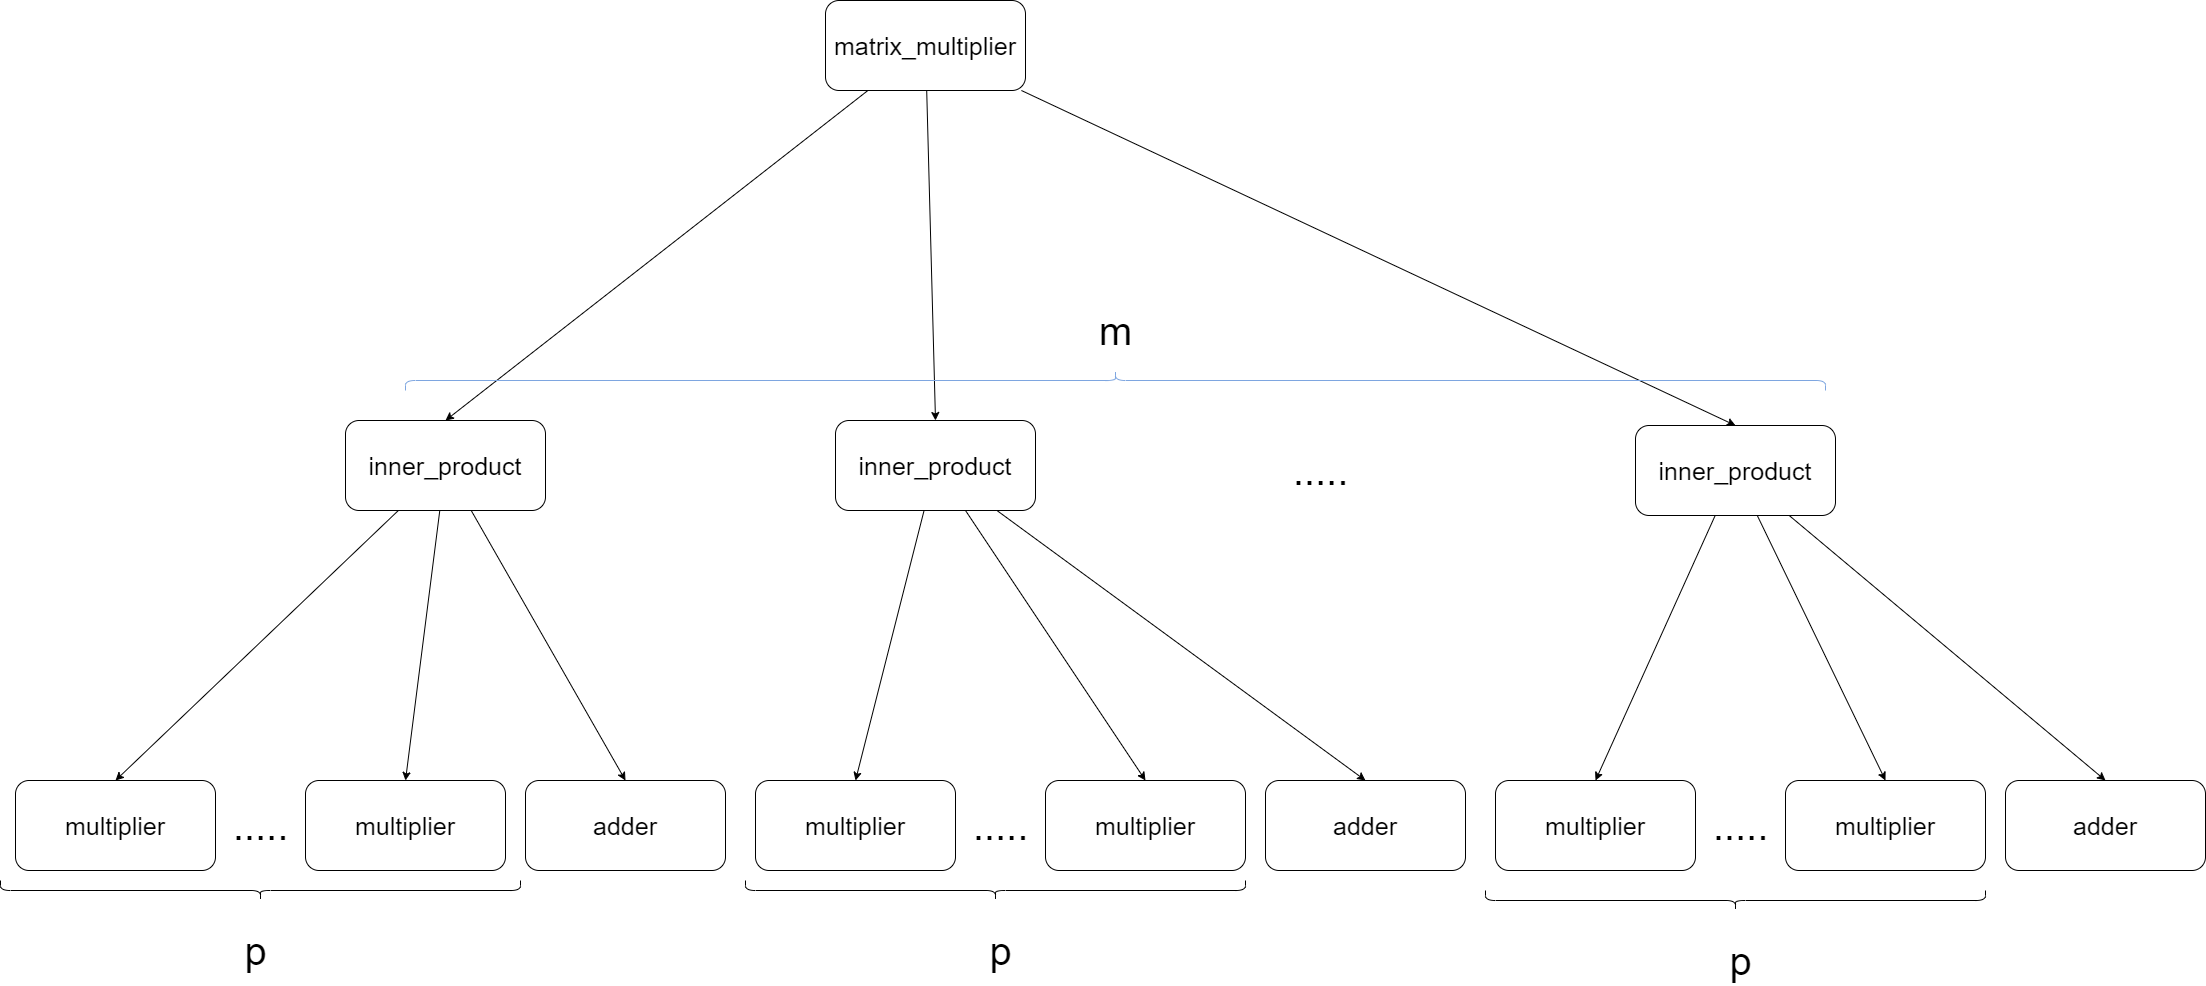
\includegraphics[scale=0.2]
    {Images/System Architecture/DSD_Project_hierarchy.png}\\
\end{center}

\newpage
\section{روند شبیه‌سازی}
\subsection{توصیف \lr{test bench} }
\subsection{\lr{test bench} ماژول \lr{adder}}
در تست این ماژول سعی شده همه‌ی حالات ممکنی که برای جمع دو عدد وجود دارد تست شود برای مثال جمع دو عدد مثبت، جمع دو عدد منفی، جمع یک عدد مثبت و یک عدد منفی و ... همچنین سعی شده حالت‌های خاص نیز پوشش داده شود برای مثال جمع دو عدد بی‌نهایت و یا جمع عدد و غیرعدد در تست‌ها لحاظ شده‌اند.
در شکل زیر خروجی تست بنچ برای ورودی‌های متفاوت مشاهده می‌شود.
\begin{center}
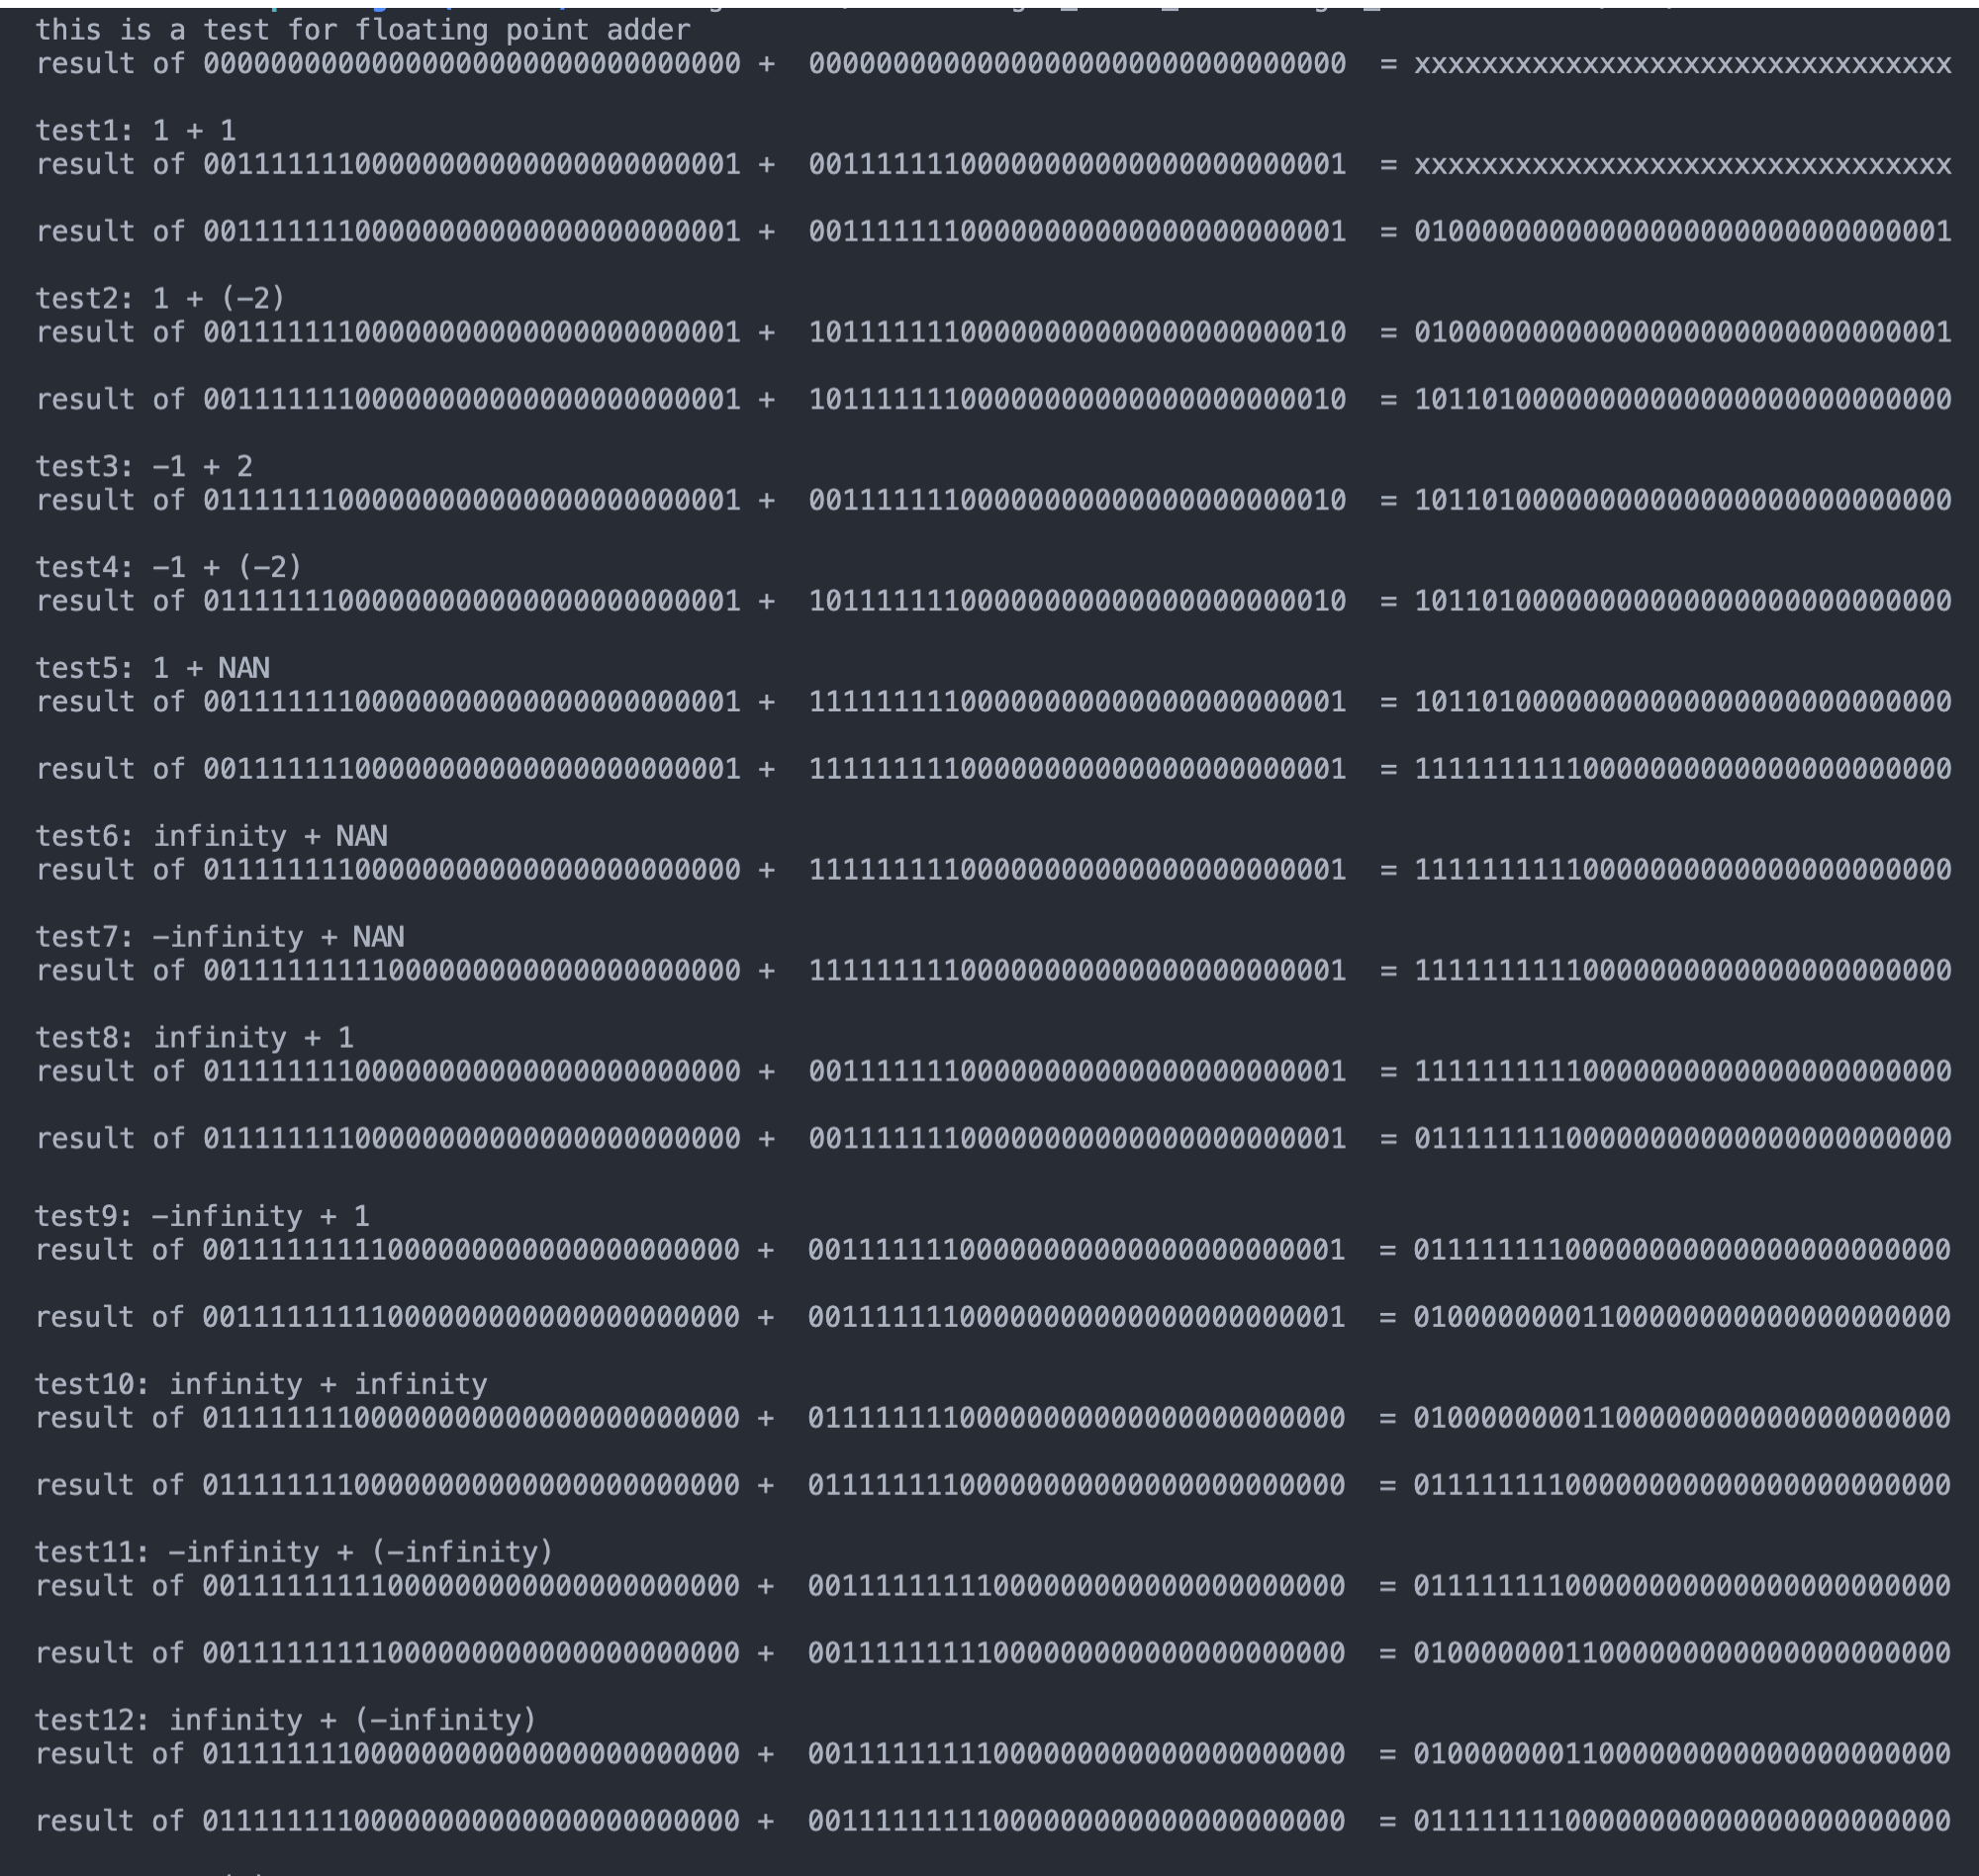
\includegraphics[scale=0.2]
    {Images/Test Bench/adder_test_bench.png}
\end{center}
\lr{wave form} به دست آمده نیز در شکل بعدی قابل مشاهده است.
\begin{center}
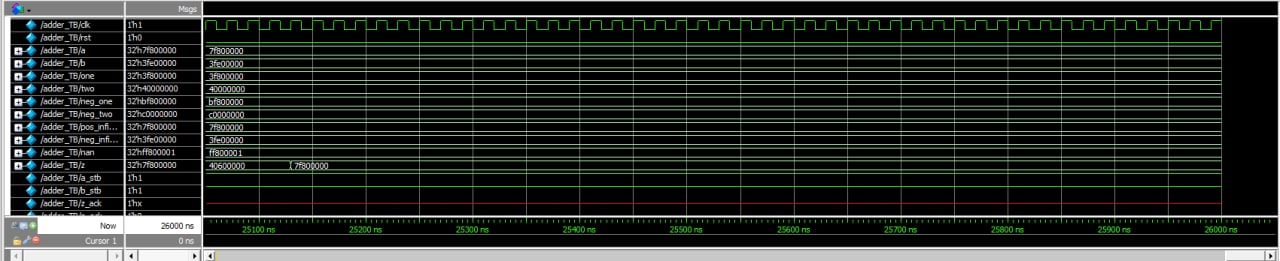
\includegraphics[scale=0.45]
    {Images/Test Bench/adder_waveform.jpg}
\end{center}

\subsection{\lr{test bench}ماژول \lr{inner product}}
در این تست بنچ با ضرب دو بردار چهار درایه ای برخی حالات لازم را ایجاد و بررسی کردیم.
در شکل زیر خروجی تست مشاهده می‌شود.
\begin{center}
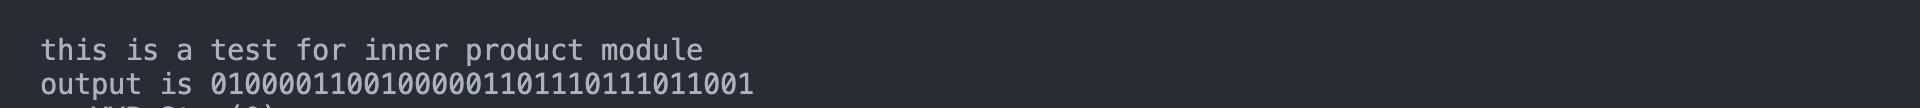
\includegraphics[scale=0.45]
    {Images/Test Bench/inner_product_test_bench.png}
\end{center}
\lr{wave form} به دست آمده نیز در شکل قابل مشاهده است.
\begin{center}
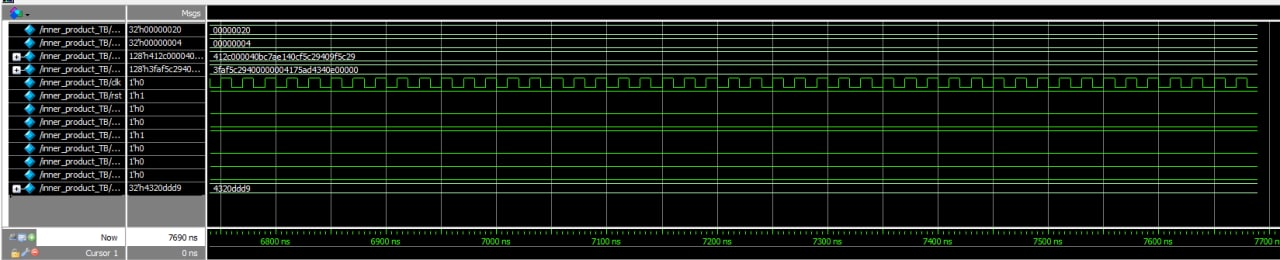
\includegraphics[scale=0.45]
    {Images/Test Bench/inner_product_waveform.jpg}
\end{center}


\subsection{\lr{test bench}ماژول \lr{matrix multiplier}}


\begin{center}
\includegraphics[scale=0.45]
    {Images/Test Bench/matrix_multiplier_test_bench.png}
\end{center}
\lr{wave form} به دست آمده نیز در شکل قابل مشاهده است.
\begin{center}
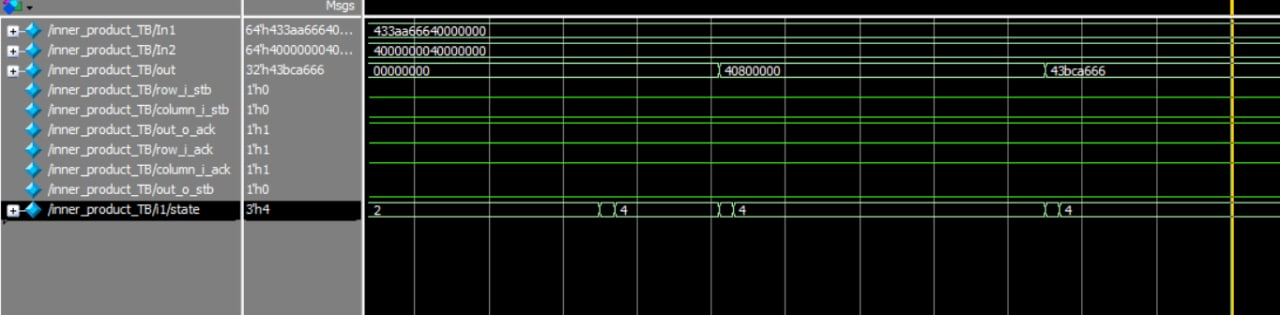
\includegraphics[scale=0.56]
    {Images/Test Bench/matrix_multiplier_waveform.jpg}
\end{center}

\newpage
\medskip


\bibliographystyle{unsrt-fa}
\bibliography{mybibliography}




\end{document}

